% !TeX spellcheck = en_GB

\section{Problem 4}

In what follows, we present the development process of our recipes search engine. We will focus on techniques and technologies we used to implement it, giving to the reader some brief explanations of key Information Retrieval (IR) concepts. You can find the source code in the material attached with this documentation.\medskip

\noindent\textbf{Disclaimer}: to run our code, be sure to be on a Linux machine (or any other that allows you to run Bash scripts) and have Python 2.7 installed. Note that some additional Python modules are required (see following sections).


\subsection{Recipes gathering}

Our initial approach was to implement a Python crawler to gather all the 11300 recipes that BBC site\cite{bbc} provides. We decided to use \textit{urllib2}\cite{urllib2} module to download .html pages containing recipes info and \textit{BeautifulSoup}\cite{beaut_soup} module to parse them and get links to other recipes.\\
Even though we succeeded in building a quite good crawler, we soon realized that this approach gave us no guarantees of downloading all recipes in the site and that it would take a lot of time to check which were the missing ones. Therefore, we looked for a better approach and found out that BBC exposes an .xml sitemap that gathers all the links to web pages of the site. At that point we were able to extract from that file all the relevant links, using \textit{BeautifulSoup}\cite{beaut_soup} utilities and regexes. You can find the code we used for this purpose in \textit{list\_recipes.py}.\\
The Python script we used was made to write recipes links to a .txt file. Then, we wrote a simple Bash script (\textit{download\_recipes.sh}) to process this file and download the recipes using \textit{wget} command. The real strength of this approach was that we were able to decide whether all recipes had been downloaded or not (due, for instance, to network issues) by checking downloaded files against the list of recipes urls (see \textit{check\_recipes.sh}).\\
To run our scripts, open a terminal and type
\begin{lstlisting}
	$ python list_recipes.py
	$ ./download_recipes.sh
\end{lstlisting}
Note that the entire download process could take more or less 4 hours to terminate. To check the result, type
\begin{lstlisting}
	$ ./check_recipes.sh
\end{lstlisting}
In case any recipe was not downloaded, the script will output the list of related urls and you can restart the download process (only for missing ones).


\subsection{Pre-processing}

In order to pre-process recipes, we first needed to extract from downloaded .html pages relevant informations.  Again, we used \textit{BeautifulSoup}\cite{beaut_soup} utilities to parse them. Then, we stored obtained info in a big .tsv file, where each row represented a recipe, using \textit{unicodecsv}\cite{csv} module. You can find the code we used for this purpose in \textit{store\_recipes.py}. To run the script, open a terminal and type
\begin{lstlisting}
	$ python store_recipes.py
\end{lstlisting}
Note that the process takes about 15 minutes to terminate. Resulting file (\textit{recipes.tsv}) should appear like in the picture below.
\begin{center}
	\vspace{5mm}
	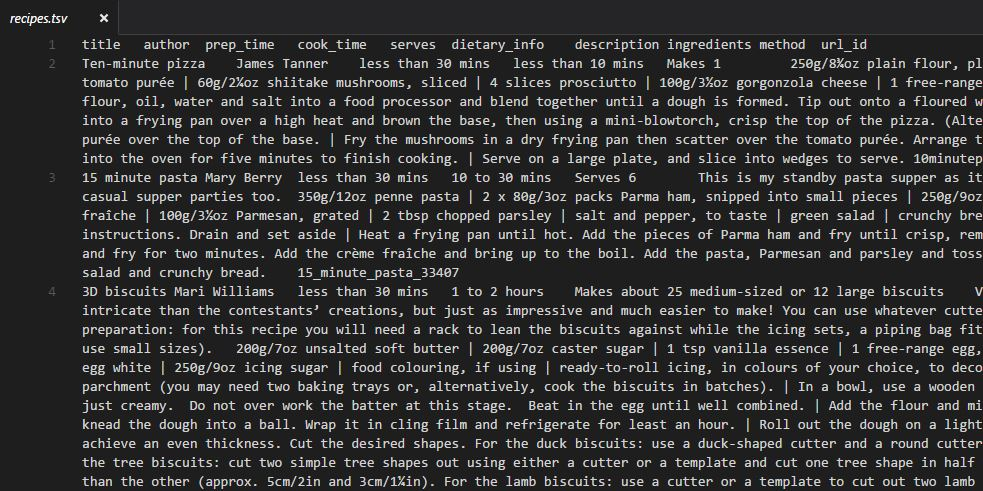
\includegraphics[scale=0.5]{img/recipes-tsv.jpg}
\end{center}
On that result, we applied pre-processing techniques (re-using parts of the \textit{NLTK}\cite{nltk} library). We created a separated Python module (named \textit{preprocessing.py}) encapsulating all pre-processing logic, to be able to reuse it also in query processing part. In particular, this module includes functions implementing:
\begin{itemize}
	\item Tokenization
	\item Normalization
	\begin{itemize}
		\item remove diacritics.
		\item remove non-alphanumeric characters (optional).
		\item convert text to lowercase.
		\item convert special unicode characters (e.g. fractions) into a somewhat "equivalent" ASCII representation.
	\end{itemize}
	\item Stopwords removal
	\item Stemming (optional)
\end{itemize}
Then, we made another script to store pre-processing results into another big .tsv file. You can find the code we used for this purpose in \textit{preprocess\_recipes.py}. To run the script, open a terminal and type
\begin{lstlisting}
	$ python preprocess_recipes.py
\end{lstlisting}
Resulting file (\textit{recipes-prep.tsv}) should appear like in the picture below.
\begin{center}
	\vspace{5mm}
	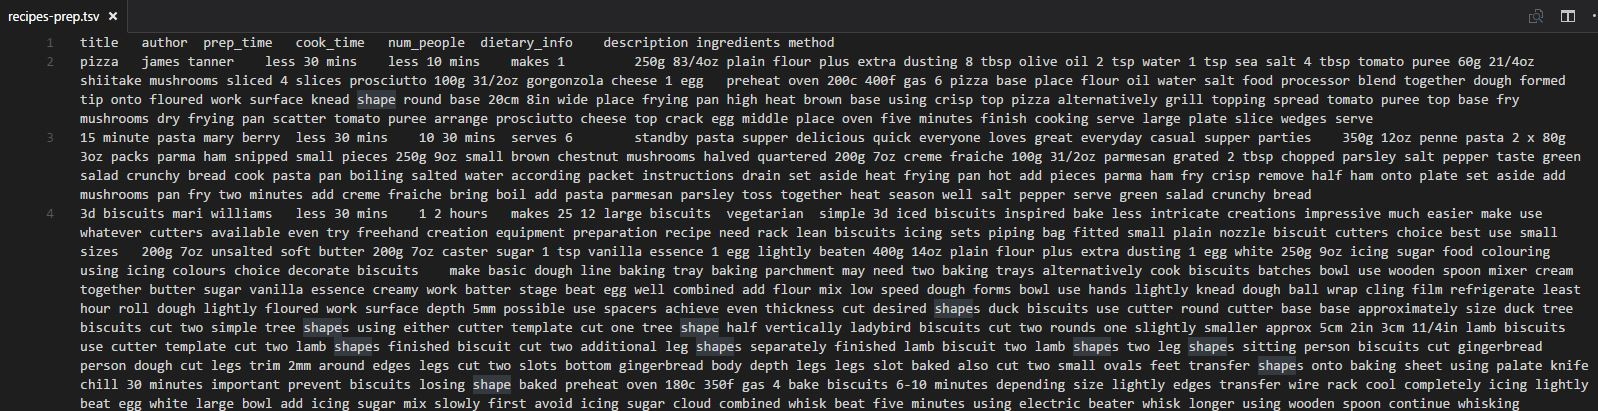
\includegraphics[scale=0.5]{img/recipes-prep-tsv.jpg}
\end{center}


\subsection{Creation of the inverted index}

An Inverted Index\cite{inv_ind} is a particular data structure storing a mapping from words in a corpus of documents to their locations (i.e. in which documents they occur). Such a structure is necessary to efficiently perform proximity queries on our recipe corpus, using the cosine-similarity measure. You can find the code we used for this purpose in \textit{build\_index.py}.\\
Basically, we developed a script that scans the whole corpus, building as you go both the doc-term (sparse) matrix\cite{doc_term} and its transpose, i.e. the index. The index is represented as a Python dictionary, in which an entry has the following structure:
\begin{center}
	\textit{term $\rightarrow postin$g list}
\end{center}
A \textit{posting} is represented as a 2-items Python list \textit{(doc\_id, tf)}, where:
\begin{itemize}
	\item \textit{doc\_id} is the document id.
	\item \textit{tf} is the term frequency (i.e. number of times term occurs) in \textit{doc\_id}.
\end{itemize}
Note that (by construction) the list is sorted with respect to \textit{doc\_id}.\\
The doc-term matrix is represented as a Python list of documents in \textit{bag-of-words} form. Each row (i.e. doc) is a sparse vector, implemented with a Python dictionary in which an entry has the following structure:
\begin{center}
	\textit{term $\rightarrow$ tf}
\end{center}
For the sake of efficiency, we made the two data structures share their entries. Indeed, matrix cells (instead of the single tf value) actually contain (a reference to) the corresponding posting in the index. Therefore, the script scans the documents in the corpus, updating as it goes the value of the \textit{tf} of the terms it encounters, and building in one shot both the matrix and the index.\\
The built doc-term matrix is later used to build an optimized version of the index for query processing, in which for each posting in a term posting list, we actually store the complete query-independent factor, i.e.
\begin{align*}
	tf_{term,doc} \cdot \dfrac{idf_{term}^2}{||doc||}
\end{align*}
where $idf_{term}$ is the Inverse Document Frequency\cite{tf_idf} of the term, and $||doc||$ is the length of the vector representing the document.\\
To run the script, open a terminal and type
\begin{lstlisting}
	$ python build_index.py
\end{lstlisting}
Finally, both the doc-term matrix and the index are dumped on the disk into separate .pickle files (we used the \textit{pickle}\cite{pickle} module to do that). This allows for easy and efficient reloading of the index in main memory at a later time (e.g. when needed for query processing).


\subsection{Query processing}

To make queries against our corpus of recipes we built a Python module (named \textit{query\_processing.py}) encapsulating all the logic and algorithms needed to process them. Then, we created a simple command line interface (\textit{process\_queries.py} module) through which we are able to submit a query and get the related recipes, presented in a structured way.\\
Note that we assumed that it was feasible to store the whole index in main memory. We are aware that this assumption doesn't hold in general, and that there exist proper algorithms and methodologies to deal with indices for extremely large corpora (e.g. external sorting algorithm, a.k.a. "k-way" merge sort). However, in our particular case, the corpus is not very big and the size of the resulting index is quite small. Indeed, we profiled the index using the \textit{pympler}\cite{pympler} module and found out that the index has a size of approximately 215 MB, making it perfectly feasible to keep it in main memory and get a more efficient query evaluation. To check the index size, a script is available: you can open a terminal and type
\begin{lstlisting}
	$ python index_size.py
\end{lstlisting}
In our initial approach to query processing we focused on \textit{disjunctive queries}. Indeed, for instance, a query like \textit{"butter apple banana"} returned the $K$ most related recipes (according to cosine-similarity) that contained \textit{at least one} of the words in the query. \\
This was trivially achieved by selecting the posting lists related to each of the terms, and \textit{merging} them, computing the score for each document (using the related query-independent factor stored in the postings), finally returning the $K$ recipes with the highest score. Some additional notes: queries are first pre-processed using the same techniques used for the recipes; document content retrieval is performed by scanning the \textit{recipes.tsv} file, collecting in a single pass only the rows of interest (using resulting document ids).\\
Since queries were answered, on average, in the order of the tenth of a second, we were satisfied about the performance of the system, and decided not to perform further optimizations but instead proceed to implement some extra features.


\subsubsection{Advanced features}

We decided to extend our search engine capabilities, by also allowing \textit{term \textbf{conjunction} and \textbf{negation}}. In order to do that, we introduced some operators, denoted by sequences of special characters, and a precise syntax to use them. In the end, the following was the format of queries admitted by our system
\begin{align*}
	\text{t1 t2 }\ldots \ [ \ || \text{ t3 t4 } \ldots \ || \ \ldots \ ] \ [ \text{ *vegetarian } | \text{ *vegan } | \text{ *lactose-int }] \ [ \text{ -t5 -t6 }\ldots \ ]
\end{align*}
Terms separated only by a blank space are assumed to be in conjunction. Blocks surrounded by square brackets are optional. The operators we introduced are:
\begin{itemize}
	\item $||$ , disjunction operator. Sequences of terms separated by this operator are assumed to be in disjunction.
	
	\item $-$ , negation operator. Terms preceded by this operator should not appear in resulting documents.
	
	\item $*$ , keyword operator. This operator introduces keywords of our system. The result of a keyword evaluation is its substitution with a sequence of predefined negated terms. This trick then lets us support \textit{\textbf{diet-aware queries}}, reducing them to a simple pruning of the resulting recipes.
\end{itemize}
To process this type of queries, we parse the textual query, extracting the conjunctive groups (i.e. groups of terms in \textit{and}), and the negated terms. Each conjunctive group is processed individually, iteratively applying the \textit{"merging intersect algorithm"} described in \cite{iir} (ch. 1, pag. 11). Then, to compute the disjunction, a simple \textit{"merging union algorithm"} is applied (keeping for each doc only its highest score). Finally, we prune the result using a \textit{"merging subtraction algorithm"}, removing those documents that contain negated terms.

\medskip

\noindent Then, we introduced \textit{\textbf{field-aware term weighting}}, modulating the weight of each term in the bag-of-words representation of a recipe according to the particular "field" of the recipe it occurs in (intuitively, a term appearing in the title is more relevant than the same term occurring in the method, and is therefore given a larger weight).

\medskip

\noindent As a last addition, we developed a simple \textbf{\textit{web interface}} for the search engine using the \textit{Flask}\cite{flask} microframework. From the home page, you can type a query and get a nicely formatted list of the corresponding most related recipes. Clicking on a particular recipe redirects you to the related page on the BBC site\cite{bbc}.
\begin{center}
	\vspace{5mm}
	
\includegraphics[scale = 0.5]{img/homepage.jpg}
\end{center}


\subsubsection{Instructions to run}

To run the command line interface, open a terminal and type
\begin{lstlisting}
	$ python process_queries.py
\end{lstlisting}
Then, follow the format specified in the previous section to input a legal query. You can exit the program by simply pressing Enter without inserting text (or forcing process termination as well).

\bigskip

\noindent To run the webapp (locally), open a terminal and type
\begin{lstlisting}
	$ python webapp.py
\end{lstlisting}
Then, open a browser and go to \url{localhost:5000}  (note that you still need a working Internet connection to view the recipes on the BBC site\cite{bbc}).

\newpage
\subsubsection{Examples}

\begin{itemize}
	\item "roast chicken and potatoes"
	\begin{center}
		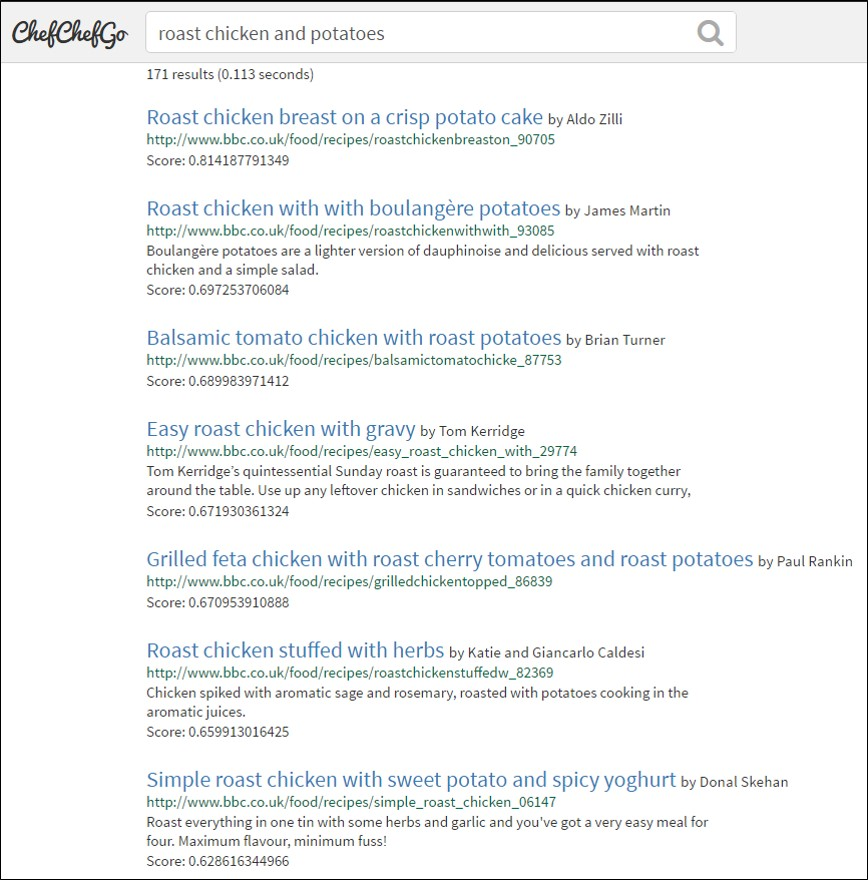
\includegraphics[scale = 0.5]{img/query1.jpg}
	\end{center}
	
	\item "roast chicken $||$ potatoes"
	\begin{center}
		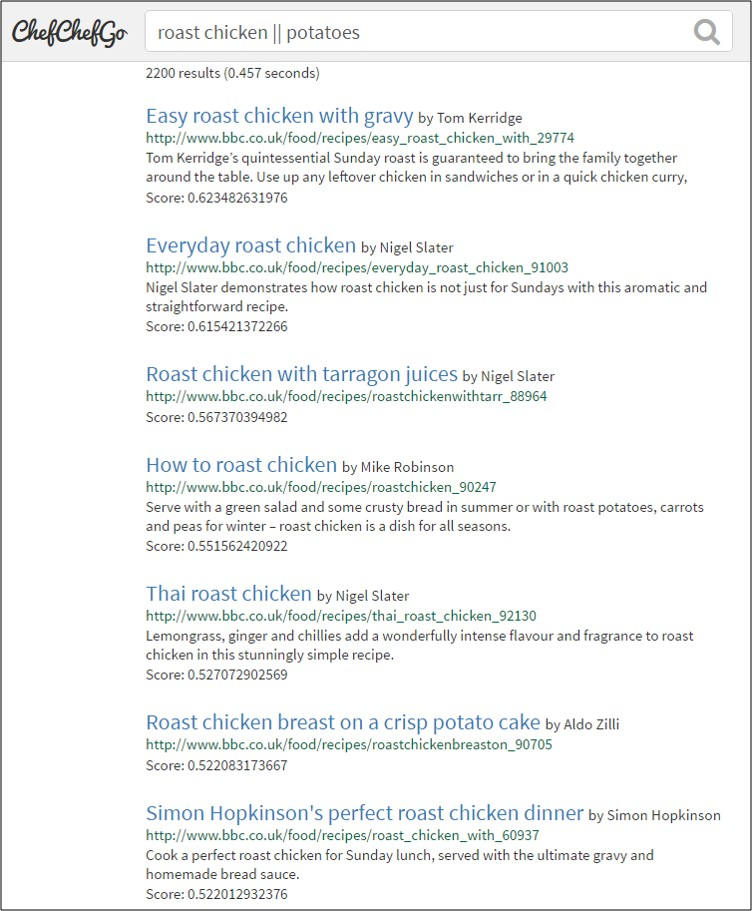
\includegraphics[scale = 0.5]{img/query2.jpg}
	\end{center}

	\item "chocolate dessert 10 minutes -peanuts"
	\begin{center}
		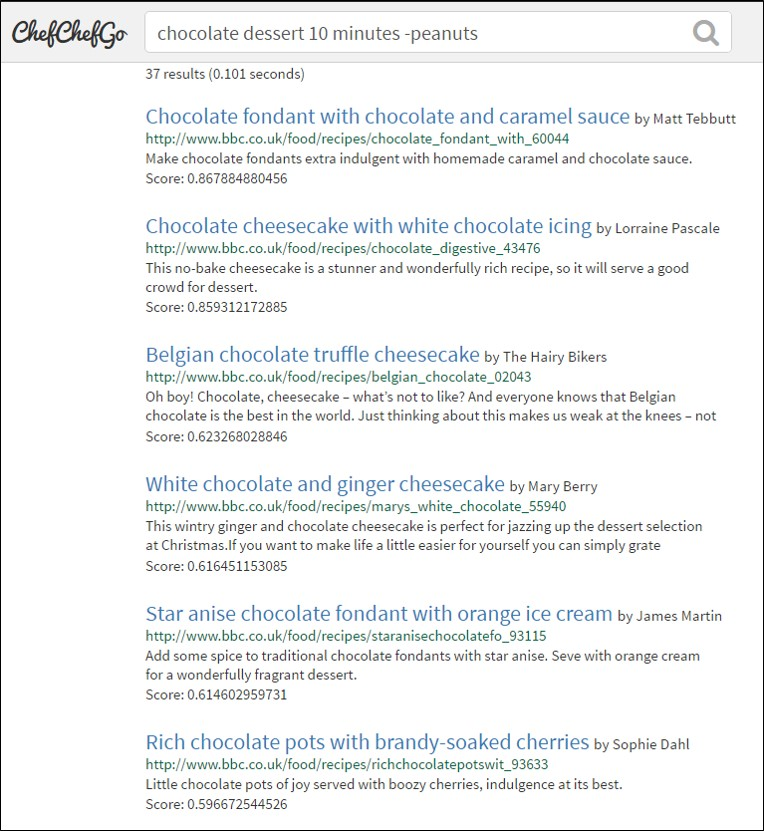
\includegraphics[scale = 0.5]{img/query3.jpg}
	\end{center}

	\item "spaghetti *vegetarian"
	\begin{center}
		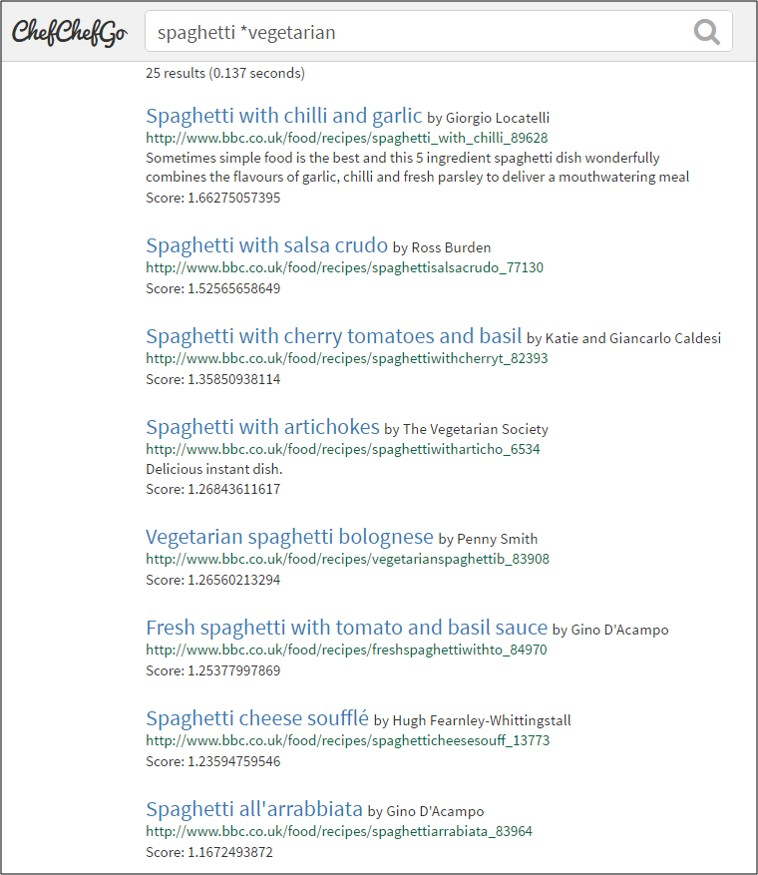
\includegraphics[scale = 0.5]{img/query4.jpg}
	\end{center}

	\item "parmigiana $||$ lasagne $||$ cannelloni *vegetarian -artichokes"
	\begin{center}
		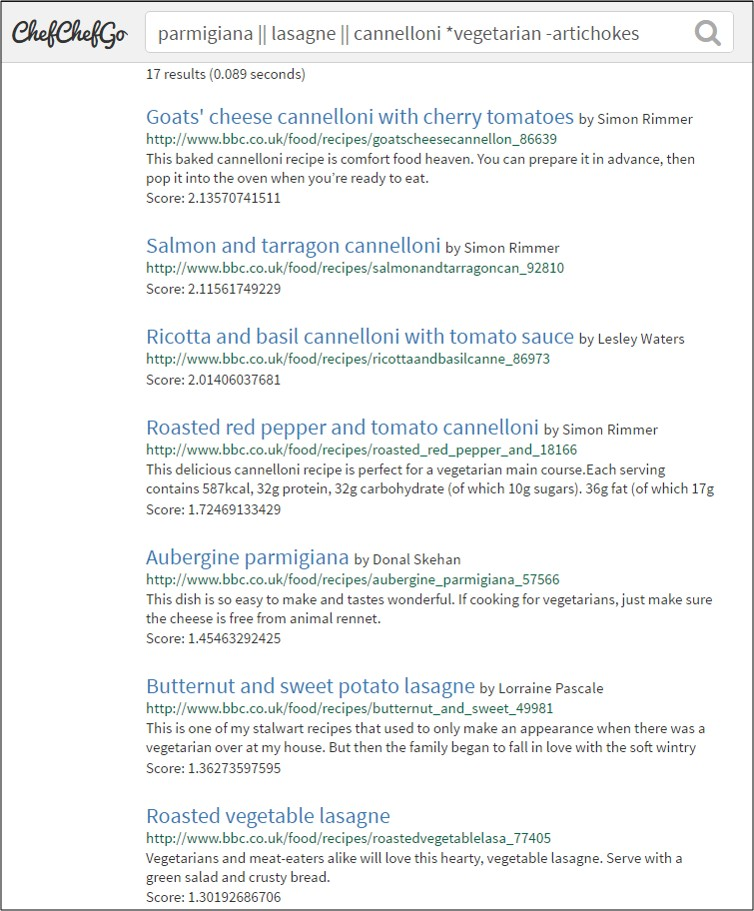
\includegraphics[scale = 0.5]{img/query5.jpg}
	\end{center}	
\end{itemize}
